%chargedCorrBtoLambdaPlots
%!TEX root = ../main.tex
%

\subsection{$B^- \rightarrow \Lambda_c^+$ decays: additional plots}
%\section{$B^- \rightarrow \Lambda_c^+$ decays: additional plots}%\label{}
\label{sec:chargedBtoLamApp}



\begin{figure}[H]
  \begin{subfigure}{15cm}
    \centering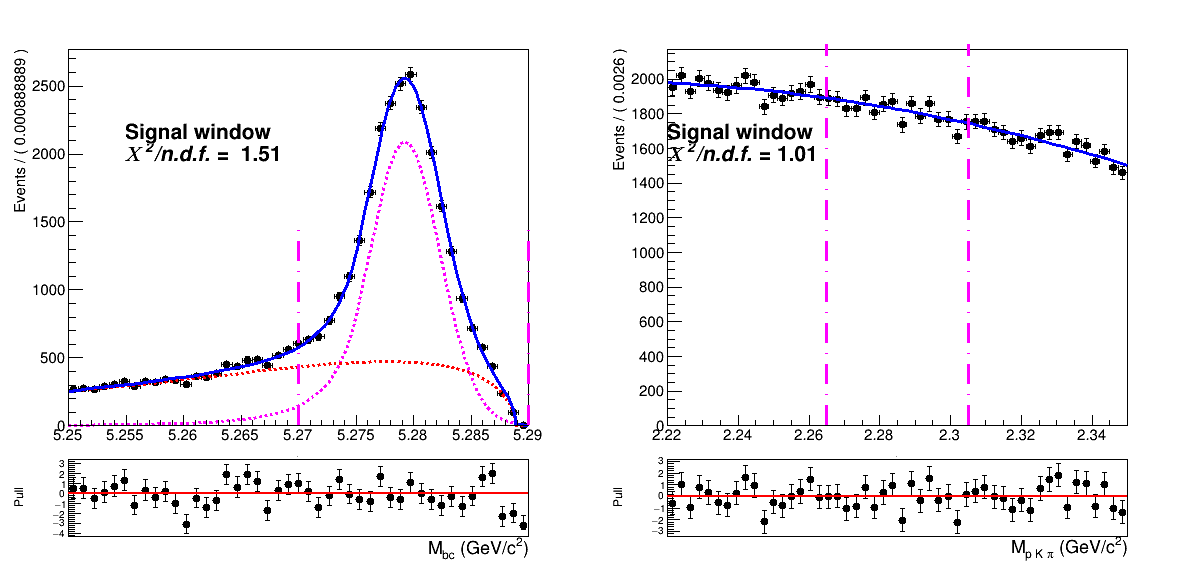
\includegraphics[width=14cm]{A1-Appendix/figs/Signal_window_streams12345_Generic_charged_corrLambdaC_2Dfit.png}
   % \caption{Fit on $M(p K \pi)$ in the region $5.25 < M_{bc} < 5.258$ GeV/c$^2$.  }
   % \label{fig:CrossfeedMbcRegionsInvMpeak1}
  \end{subfigure}
  \begin{subfigure}{15cm}
    \centering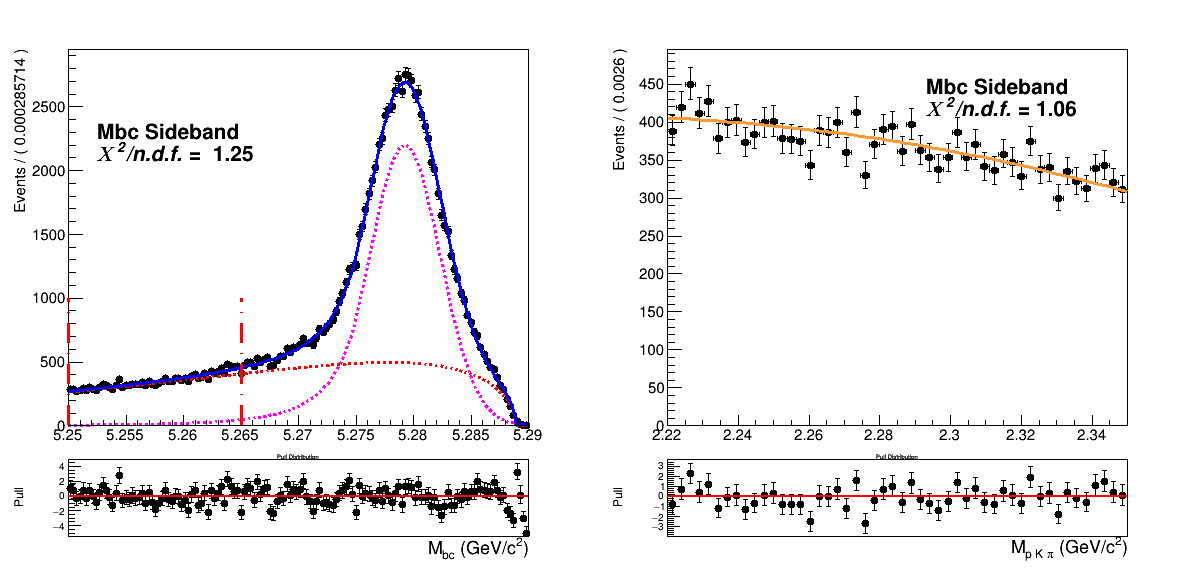
\includegraphics[width=14cm]{A1-Appendix/figs/Mbc_Sideband_stream12345_Generic_charged_corrLambdaC_2Dfit.png}
  \end{subfigure}

  \begin{subfigure}{15cm}
    \centering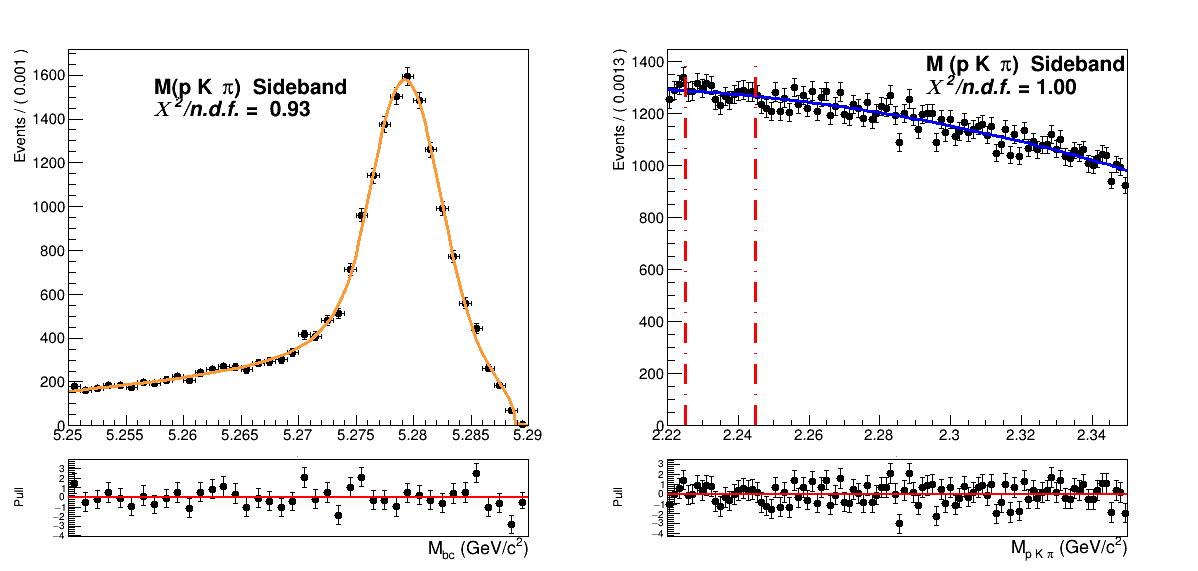
\includegraphics[width=14cm]{A1-Appendix/figs/InvM_Sideband_stream12345_Generic_charged_corrLambdaC_2Dfit.png}
  \end{subfigure}
  \caption{Signal region and sidebands of the two dimensional fit of generic background shown in \cref{fig:5streams_Generic_charged_corrLambdaC_2Dfit}}
\end{figure}


\newpage


\begin{figure}[H]
  \begin{subfigure}{15cm}
    \centering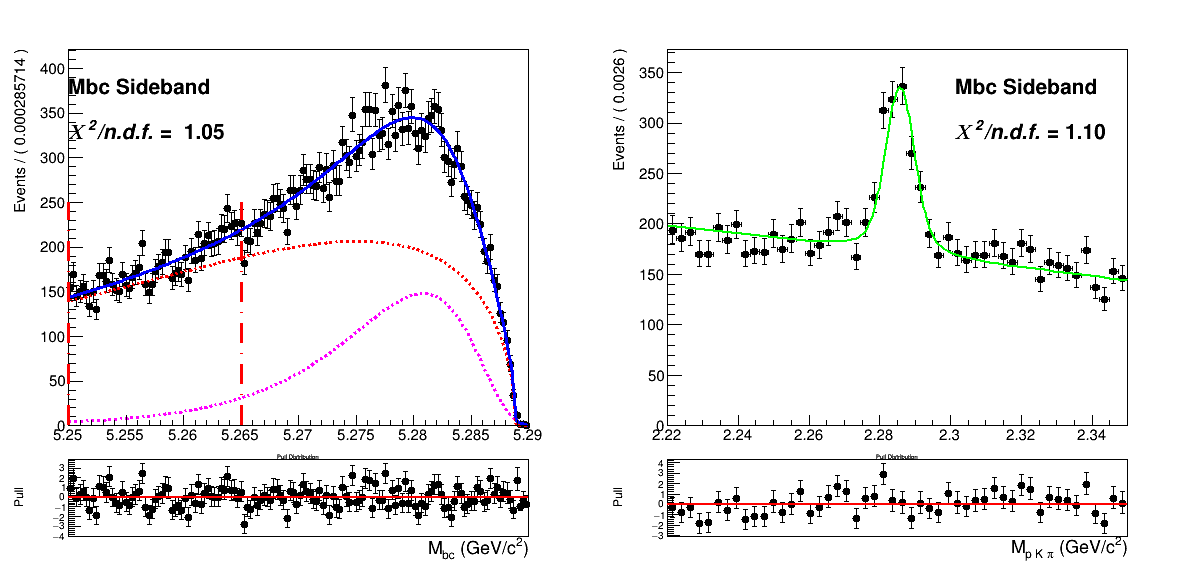
\includegraphics[width=14cm]{A1-Appendix/figs/Mbc_Sideband_stream12345_Crossfeed_charged_corrLambdaC_2Dfit_afterParametrization.png}
   % \caption{Fit on $M(p K \pi)$ in the region $5.25 < M_{bc} < 5.258$ GeV/c$^2$.  }
   % \label{fig:CrossfeedMbcRegionsInvMpeak1}
  \end{subfigure}
  \begin{subfigure}{15cm}
    \centering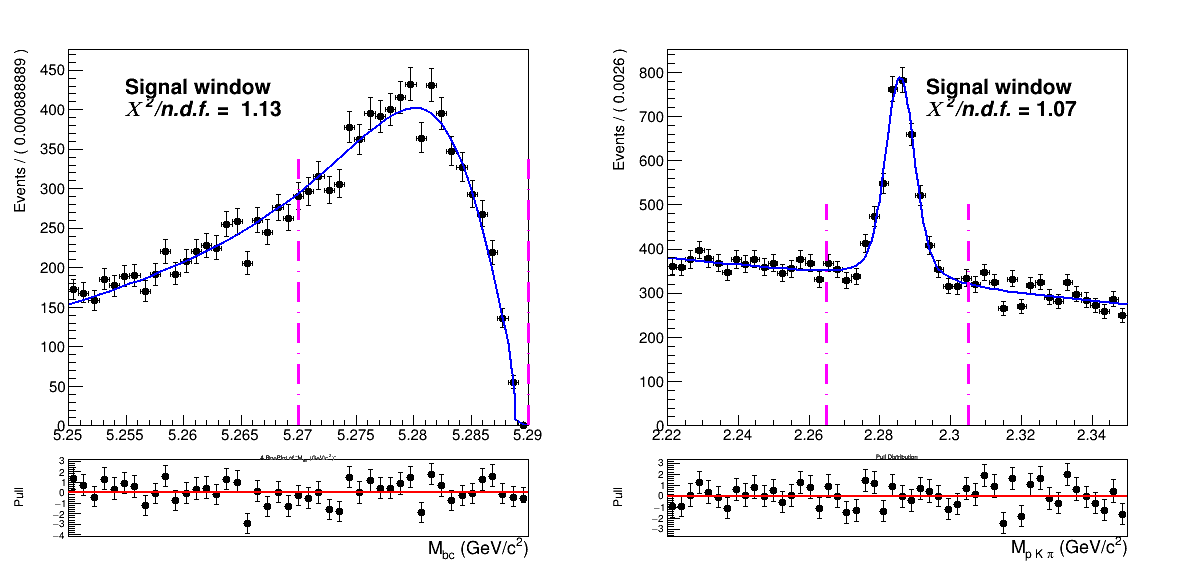
\includegraphics[width=14cm]{A1-Appendix/figs/Signal_window_stream12345_Crossfeed_charged_corrLambdaC_2Dfit_afterParametrization.png}
  \end{subfigure}

  \begin{subfigure}{15cm}
    \centering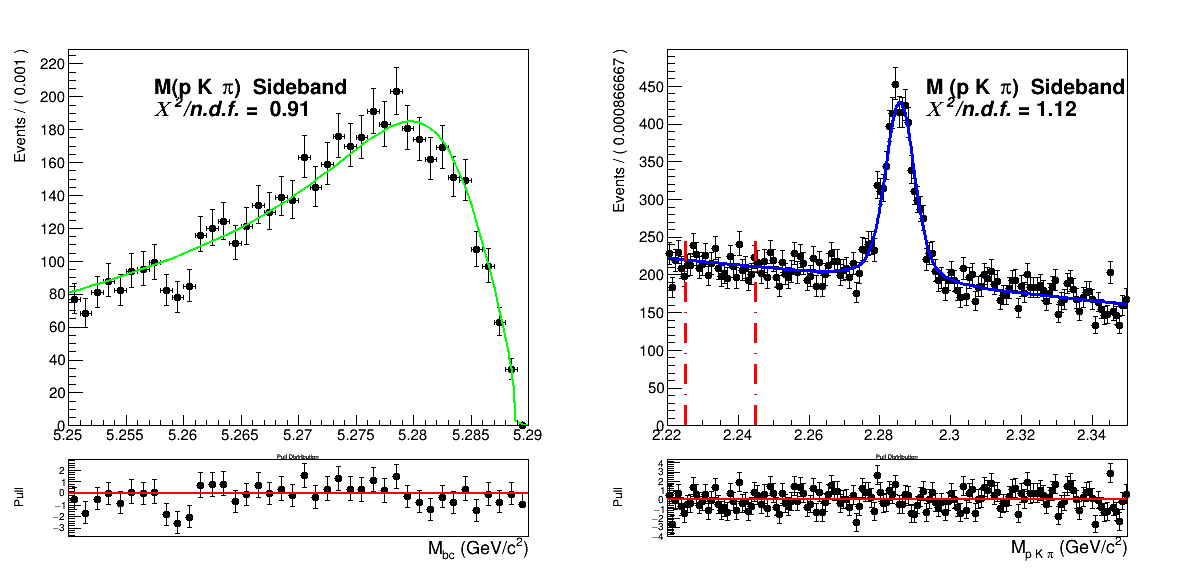
\includegraphics[width=14cm]{A1-Appendix/figs/InvM_Sideband_stream12345_Crossfeed_charged_corrLambdaC_2Dfit.png}
  \end{subfigure}
  \caption{Signal region and sidebands of the two dimensional fit of crossfeed background after parametrization}
\end{figure}

\newpage


\begin{figure}[H]
  \begin{subfigure}{15cm}
    \centering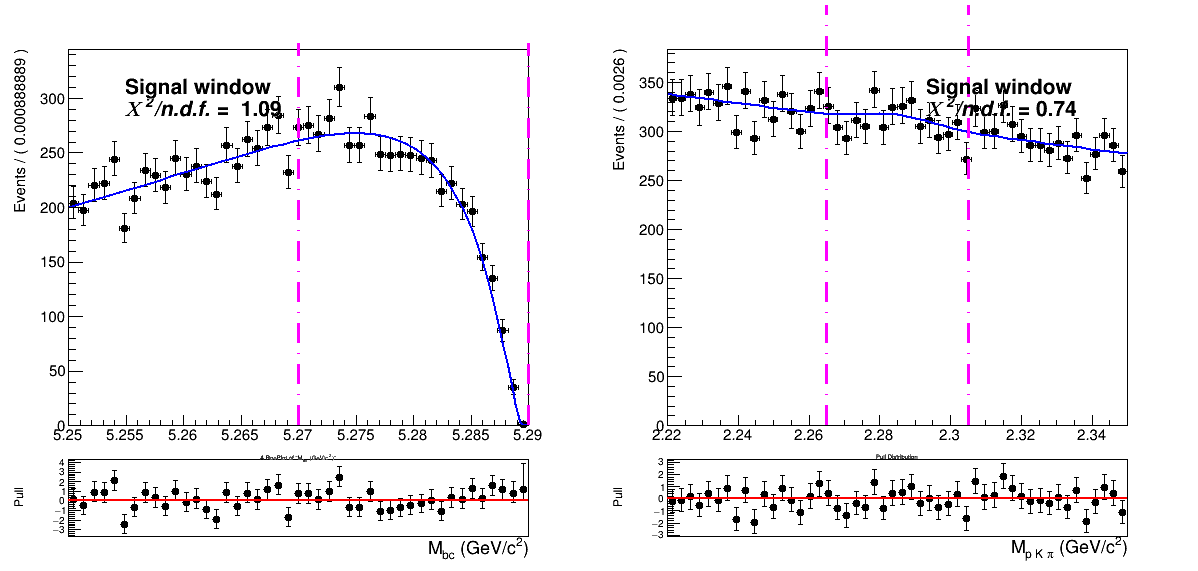
\includegraphics[width=14cm]{A1-Appendix/figs/Signal_window_stream3_Continuum_charged_corrLambdaC_2Dfit.png}
   % \caption{Fit on $M(p K \pi)$ in the region $5.25 < M_{bc} < 5.258$ GeV/c$^2$.  }
   % \label{fig:CrossfeedMbcRegionsInvMpeak1}
  \end{subfigure}
  \begin{subfigure}{15cm}
    \centering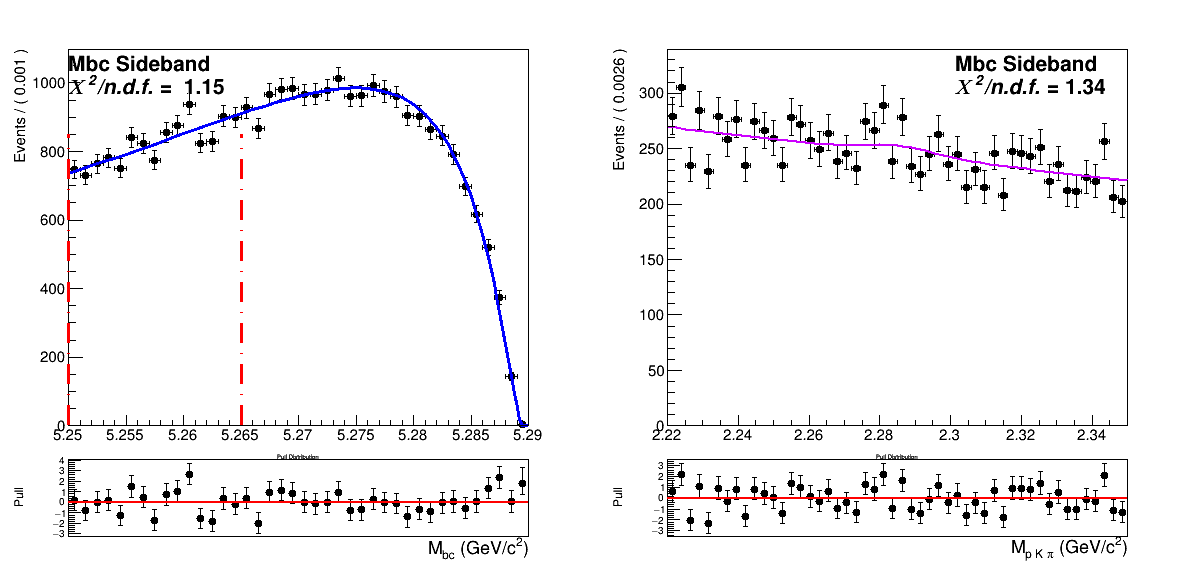
\includegraphics[width=14cm]{A1-Appendix/figs/Mbc_Sideband_stream3_Continuum_charged_corrLambdaC_2Dfit.png}
  \end{subfigure}

  \begin{subfigure}{15cm}
    \centering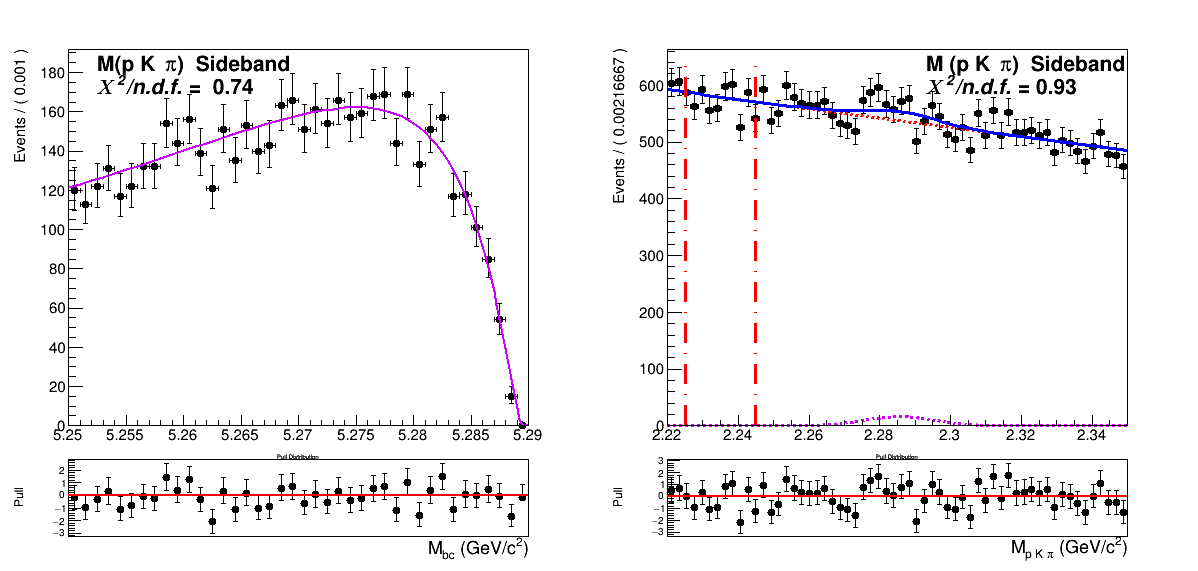
\includegraphics[width=14cm]{A1-Appendix/figs/InvM_Sideband_stream3_Continuum_charged_corrLambdaC_2Dfit.png}
  \end{subfigure}
  \caption{Signal region and sidebands of the two dimensional fit of continuum background shown in \cref{fig:stream3corrLambddaC_total_continuum_2DFit}}
\end{figure}




\newpage

\begin{figure}[h!]
%\centering
{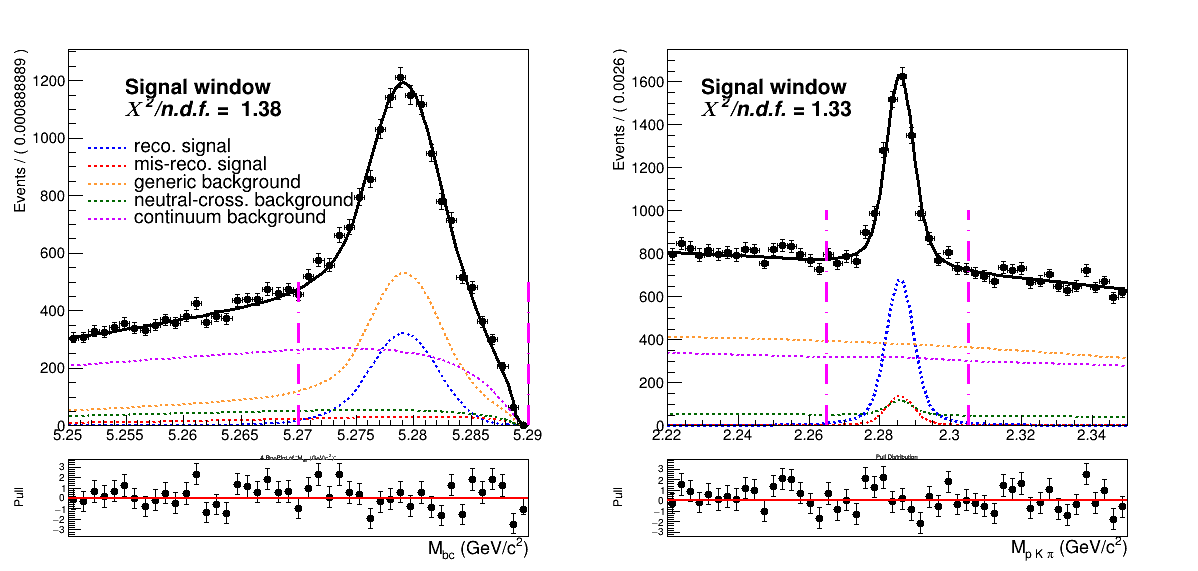
\includegraphics[width=0.75\textwidth]{A1-Appendix/figs/Signal_window_Total_2DFit_stream0_free_sigmas_free_sigmas.png}}
\caption{Signal region ($2.22 < M(p K \pi) < 2.35$ GeV/c$^2$ and $5.27 < M_{bc} < 5.29$ GeV/c$^2$ ) projections pf the dimensional fit on stream 0 Monte Carlo simulated data.}
\label{fig:stream0_sig_window_Total2Dfit_charged_corrLambdaC}
\end{figure}

\begin{figure}[h!]
%\centering
{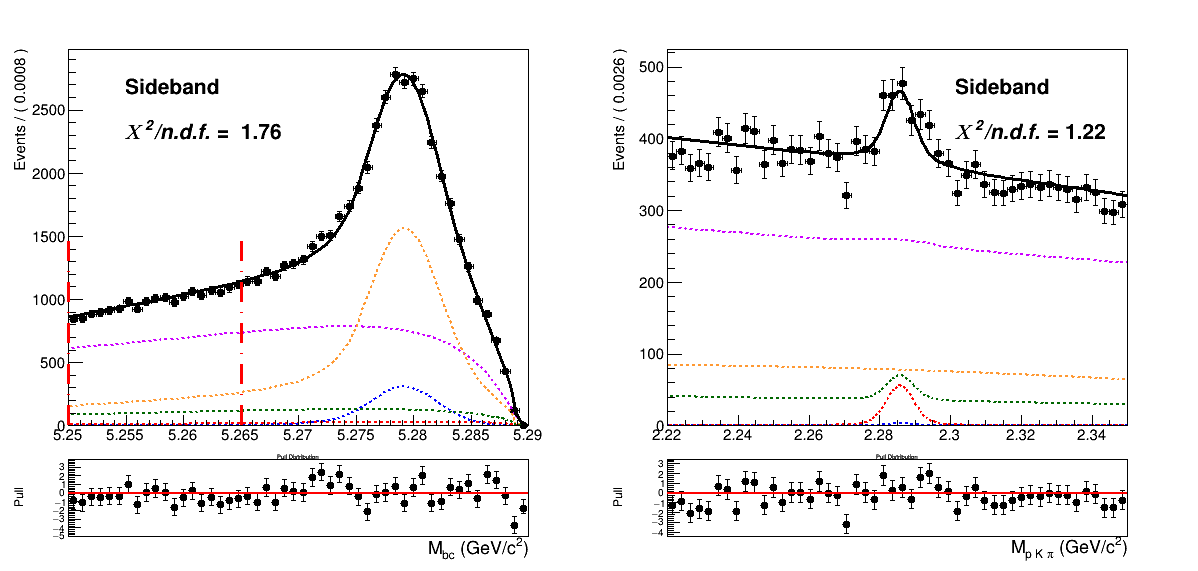
\includegraphics[width=0.75\textwidth]{A1-Appendix/figs/Mbc_Sideband_Total_2DFit_stream0_free_sigmas.png}}
\caption{Sideband region of $5.25 < M_{bc} < 5.265$ GeV/c$^2$ projection of the two dimensional fit on stream 0 Monte Carlo simulated data.}
\label{fig:stream0_MbcSideband_Total2Dfit_charged_corrLambdaC}
\end{figure}

\begin{figure}[b]
%\centering
{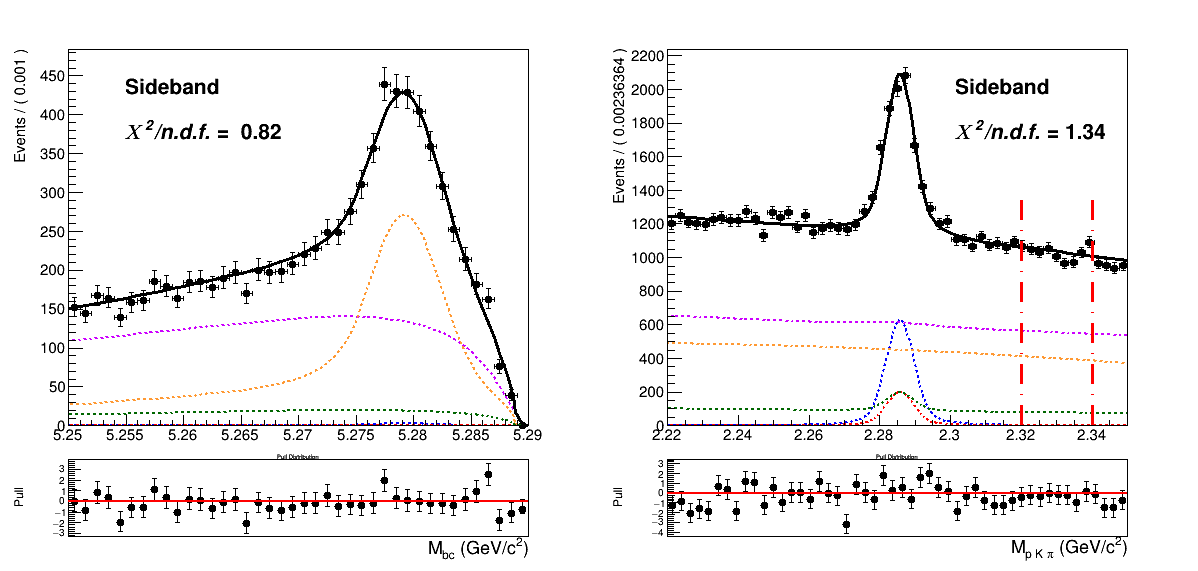
\includegraphics[width=0.75\textwidth]{A1-Appendix/figs/InvM_Sideband_Total_2DFit_stream0_free_sigmas.png}}
\caption{Sideband region of $2.22 < M(p K \pi) < 2.35$ GeV/c$^2$ projection of the two dimensional fit on stream 0 Monte Carlo simulated data.}
\label{fig:stream0_InvMSideband_Total2Dfit_charged_corrLambdaC}
\end{figure}

\newpage

\begin{figure}[h!]
  \begin{subfigure}{15cm}
    \centering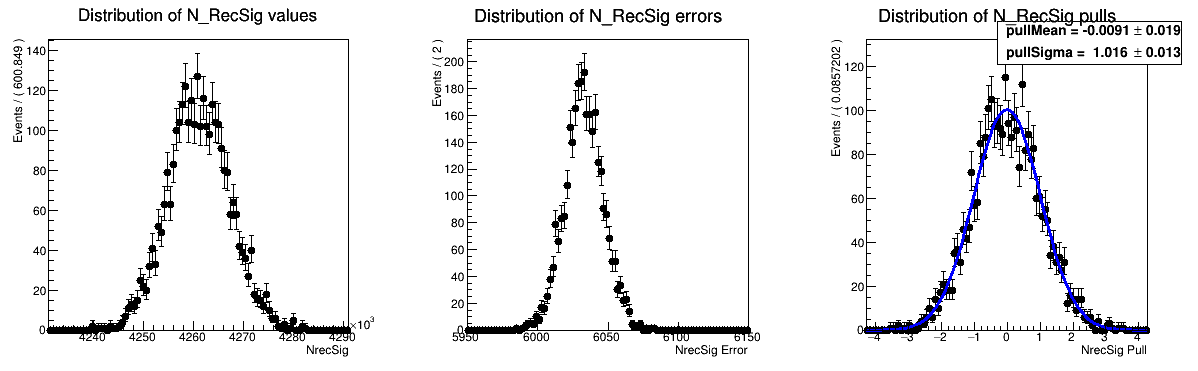
\includegraphics[width=14cm]{A1-Appendix/figs/NrecSigBtag_mcstudy.png}
   % \caption{Fit on $M(p K \pi)$ in the region $5.25 < M_{bc} < 5.258$ GeV/c$^2$.  }
   % \label{fig:CrossfeedMbcRegionsInvMpeak1}
  \end{subfigure}
  \begin{subfigure}{15cm}
    \centering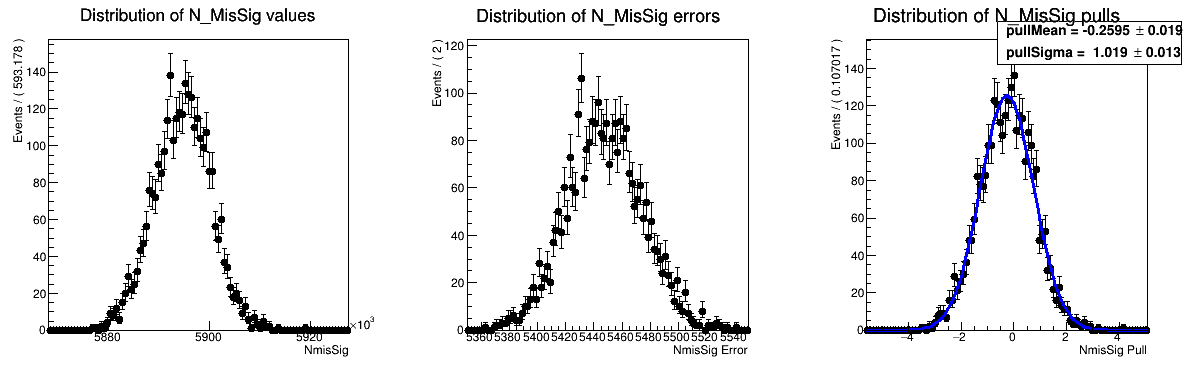
\includegraphics[width=14cm]{A1-Appendix/figs/nMisSig_mcstudy.png}
  \end{subfigure}

  \begin{subfigure}{15cm}
    \centering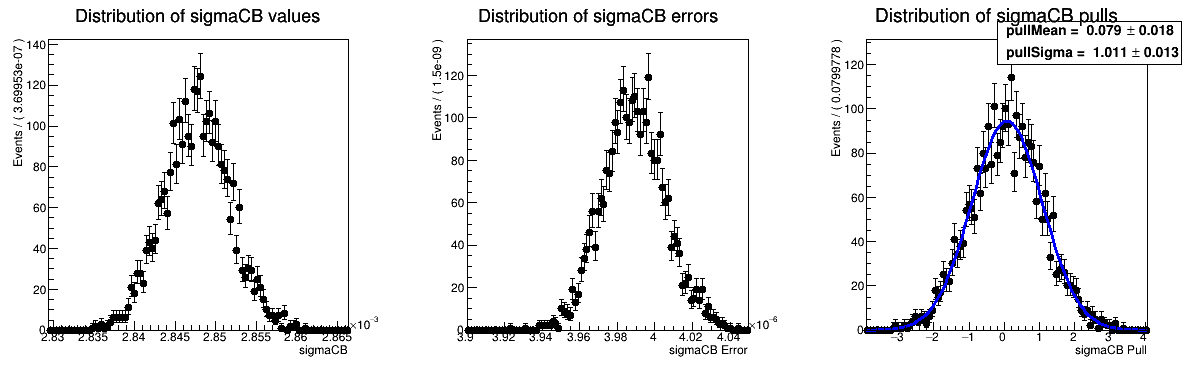
\includegraphics[width=14cm]{A1-Appendix/figs/sigmaCB_mcstudy.png}
  \end{subfigure}
  \begin{subfigure}{15cm}
    \centering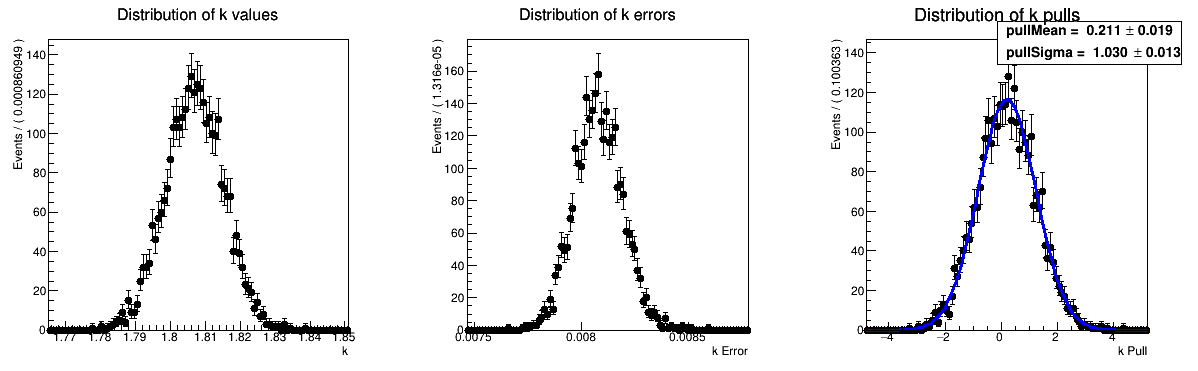
\includegraphics[width=14cm]{A1-Appendix/figs/k_mcstudy.png}
    %\label{fig:CrossfeedMbcRegionsInvMpeak5}
  \end{subfigure}
  %\label{fig:CrossfeedMbcRegionsInvMpeak}
  \caption{Toy MC study for the $B_{tag}$ fit model described in Sec. \ref{BtagFit}}
\end{figure}

